\chapter{Entropía de los agujeros negros, holografía y espacio de de Sitter}

\lectureoverview{Completamos el argumento de correspondencia iniciado en la clase anterior. La entropía de una cuerda muy excitada es proporcional a su masa, mientras que la de un agujero negro de Schwarzschild es proporcional a su área. Las dos fórmulas no se relacionan identificando un agujero negro con gravedad intensa con una cuerda libre, sino variando lentamente el acoplamiento de cuerda hasta que ambas descripciones coincidan. La ley del área conduce entonces de forma natural al principio holográfico. En la parte final de la clase se introduce el espacio en expansión y la geometría de de Sitter, cuyo horizonte estudiaremos en la siguiente clase.}

\section{Volvamos al problema de contar}

Quedaba un cabo suelto en el recuento de cuerdas largas. Si se reparte una longitud total fija entre varias cuerdas, las cuerdas idénticas de la misma longitud son indistinguibles. Sin embargo, sus posiciones en la caja forman parte del estado, y se elige una caja cuyo tamaño sea aproximadamente el de la región que ocupa la correspondiente cuerda larga individual.

\begin{classroomqa}
\audiencequestion{¿Las cuerdas cortas se distinguen unas de otras? ¿Se cuentan sus posiciones?\lecturetimestamp{00:00:37}}
\lecturerresponse{Las cuerdas con propiedades idénticas son indistinguibles, pero sus posiciones en la caja sí se cuentan. La comparación se hace a volumen fijo, elegido para que coincida con la región que ocupa la cuerda larga.}
\end{classroomqa}

Una vez aclarado esto, podemos enunciar el objetivo. Reuniremos una breve lista de ecuaciones y las usaremos para obtener la dependencia de la entropía de los agujeros negros. No hacen falta integrales ni sumas infinitas. La dificultad no es algebraica: consiste en saber qué magnitudes se pueden comparar y en qué etapa del argumento.

\section{Unidades naturales y área de Planck}

Fijemos
\begin{equation}
c=\hbar=1,
\label{eq:l07-natural-units}
\end{equation}
pero mantengamos explícita la constante de Newton. La primera consecuencia es que el tiempo y la longitud tienen las mismas unidades. La relación del fotón
\begin{equation}
E=\frac{\hbar c}{\lambda}
\end{equation}
y la relación entre masa y energía \(E=mc^2\) implican entonces
\begin{equation}
[M]=L^{-1}.
\label{eq:l07-mass-dimension}
\end{equation}
Por tanto, la masa puede expresarse como el inverso de una longitud.

\begin{figure}[htbp]
\centering
\includegraphics[width=0.62\textwidth]{lecture_07_figure_02.png}
\caption{Convención de unidades naturales al comienzo del argumento dimensional. La fórmula de la energía se completa en las ecuaciones anteriores.}
\lectureframe{00:03:27.900}
\end{figure}

Para determinar las unidades de \(G_N\), usemos la aceleración newtoniana solo como recurso para llevar la cuenta dimensional:
\begin{equation}
a\sim\frac{G_NM}{R^2}.
\end{equation}
Como \(T\) y \(L\) tienen las mismas unidades, \([a]=L/T^2=L^{-1}\). Junto con la ecuación~\eqref{eq:l07-mass-dimension}, esto da
\begin{equation}
[G_N]=L^2.
\end{equation}
En estas unidades, la constante de Newton tiene dimensiones de área. Si definimos la longitud de Planck como
\begin{equation}
G_N=\ell_p^2,
\label{eq:l07-planck-area}
\end{equation}
se entiende enseguida por qué \(A/G_N=A/\ell_p^2\) es adimensional: mide un área en unidades de áreas de Planck.

\section{El acoplamiento de cuerda y la intensidad de la gravedad}

Ahora debemos expresar la gravedad en términos de cuerdas. La imagen útil es la de un proceso de intercambio. Cuando una cuerda se cruza consigo misma, puede dividirse y volver a unirse. Un objeto puede emitir un pequeño bucle de cuerda cerrada y otro absorberlo; si esa excitación es un gravitón, el proceso media la interacción gravitatoria. En la emisión aparece un factor de interacción y en la absorción aparece otro, así que la intensidad del intercambio incluye \(g_s^2\).

El acoplamiento \(g_s\) es adimensional. Más precisamente, es un acoplamiento a nivel de amplitud, mientras que una probabilidad o una tasa empiezan en el orden \(g_s^2\).\editorialnote{En la clase, a veces se llama probabilidad a \(g_s\) y luego se corrige esa afirmación: se trata de la raíz cuadrada de una probabilidad. El acoplamiento perturbativo corresponde al nivel de amplitud.} Como \(G_N\) tiene dimensiones de área, aún falta una escala de longitud. La longitud fundamental de cuerda \(\ell_s\), que fija la escala de una ondulación elemental de la cuerda, la proporciona:
\begin{equation}
G_N\sim g_s^2\ell_s^2,
\qquad
\ell_p\sim g_s\ell_s.
\label{eq:l07-planck-string}
\end{equation}

\begin{figure}[htbp]
\centering
\includegraphics[width=0.72\textwidth]{lecture_07_figure_05.png}
\caption{La relación entre acoplamientos escrita en la pizarra: \(G_N=\ell_p^2\) y \(g_s^2\ell_s^2\sim\ell_p^2\).}
\lectureframe{00:12:15.000}
\end{figure}

A acoplamiento débil, \(g_s\ll1\), la longitud de Planck es mucho menor que la longitud de cuerda. Reducir \(g_s\) debilita la gravedad y deja fija la escala de la cuerda elemental.\editorialnote{En una teoría efectiva de cuatro dimensiones, los datos de compactificación y las convenciones numéricas también intervienen en \(G_N\). En este argumento de escala se mantienen fijos y se omiten.}

\section{El recuento de una cuerda larga}

La entropía cuenta las decisiones elementales necesarias para especificar un estado. Reemplacemos una cuerda muy excitada por un paseo en una retícula cuadrada. En cada vértice, el siguiente enlace puede apuntar en una de cuatro direcciones. Describir la elección elemental como una decisión entre cuatro opciones o como dos decisiones binarias solo cambia una constante de orden unidad. Lo que importa es el número de pasos.

Si \(L\) es la longitud de contorno de la cuerda y cada paso tiene longitud \(\ell_s\), entonces hacen falta
\begin{equation}
N=\frac{L}{\ell_s}
\end{equation}
pasos. El número de paseos crece exponencialmente, de forma esquemática como \(\Omega_N\sim q^N\), con \(q\) de orden unidad; por tanto,
\begin{equation}
S_{\mathrm{str}}=\log\Omega_N\sim N\sim\frac{L}{\ell_s}.
\label{eq:l07-string-entropy-length}
\end{equation}

\begin{figure}[htbp]
\centering
\includegraphics[width=0.68\textwidth]{lecture_07_figure_03.png}

\vspace{0.7em}
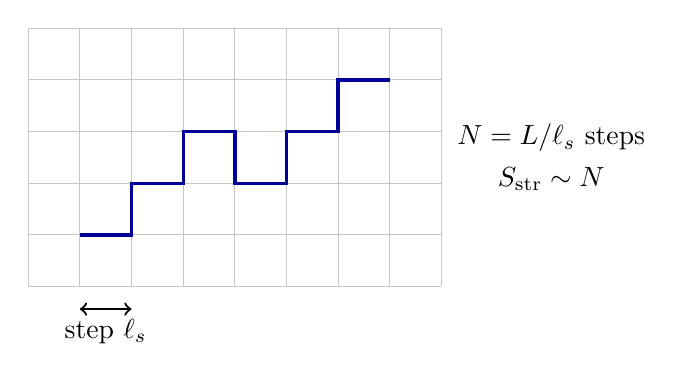
\begin{tikzpicture}[scale=0.82]
  \draw[step=0.8cm,gray!45,thin] (0,0) grid (6.4,4.0);
  \draw[very thick,blue!60!black]
    (0.8,0.8)--(1.6,0.8)--(1.6,1.6)--(2.4,1.6)--(2.4,2.4)--
    (3.2,2.4)--(3.2,1.6)--(4.0,1.6)--(4.0,2.4)--(4.8,2.4)--
    (4.8,3.2)--(5.6,3.2);
  \draw[<->,thick] (0.8,-0.35)--(1.6,-0.35);
  \node[below] at (1.2,-0.35) {step \(\ell_s\)};
  \node[align=center] at (8.1,2.0) {\(N=L/\ell_s\) steps\\[0.3em]\(S_{\mathrm{str}}\sim N\)};
\end{tikzpicture}
\caption{El modelo reticular de la pizarra y su interpretación depurada como paseo aleatorio. El número de elecciones lo determina la longitud de contorno, no el diámetro de la bola enmarañada.}
\lectureframe{00:17:20.000}
\end{figure}

La masa se cuenta a partir de los mismos segmentos elementales. Un segmento de longitud \(\ell_s\) tiene una escala de masa
\begin{equation}
m_{\mathrm{seg}}\sim\frac{1}{\ell_s}.
\end{equation}

\begin{classroomqa}
\audiencequestion{¿Se asigna al segmento elemental la longitud \(\ell_s\)?\lecturetimestamp{00:18:56}}
\lecturerresponse{Sí. Su longitud característica es \(\ell_s\), de modo que, en unidades naturales, su masa característica es \(1/\ell_s\).}
\end{classroomqa}

Al sumar las masas de los segmentos \(L/\ell_s\) se obtiene
\begin{equation}
M\sim\frac{L}{\ell_s}\frac{1}{\ell_s}
=\frac{L}{\ell_s^2},
\qquad
L\sim M\ell_s^2.
\label{eq:l07-string-mass}
\end{equation}
Esta relación de escala condensa las energías cinética y potencial de la cuerda oscilante; un tratamiento detallado de mecánica estadística da la misma dependencia. Al sustituir en la ecuación~\eqref{eq:l07-string-entropy-length} obtenemos la fórmula de la cuerda que necesitaremos:
\begin{equation}
S_{\mathrm{str}}\sim M\ell_s.
\label{eq:l07-string-entropy-mass}
\end{equation}

\begin{figure}[htbp]
\centering
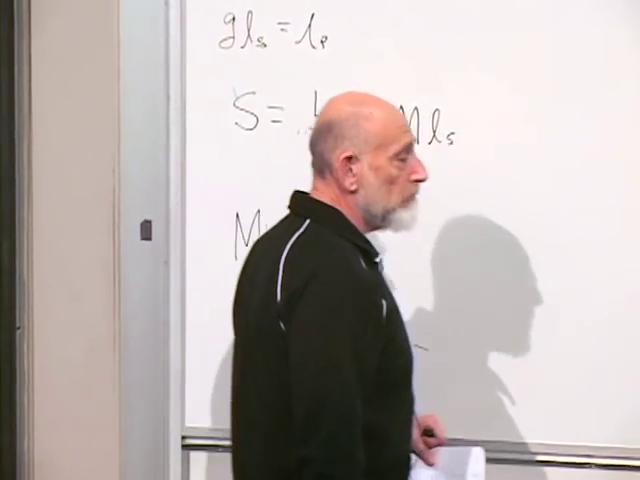
\includegraphics[width=0.66\textwidth]{lecture_07_figure_04.png}
\caption{La columna correspondiente a la cuerda, reunida antes de la comparación: \(\ell_p\sim g_s\ell_s\), \(S_{\mathrm{str}}\sim L/\ell_s\sim M\ell_s\) y \(M\sim L/\ell_s^2\).}
\lectureframe{00:21:57.800}
\end{figure}

\section{Por qué una cuerda libre todavía no es un agujero negro}

En el lado gravitatorio, la fórmula semiclásica exacta es
\begin{equation}
S_{\mathrm{BH}}=\frac{A}{4G_N}.
\label{eq:l07-bh-exact}
\end{equation}

\begin{classroomqa}
\audiencequestion{¿Qué coeficiente numérico va en el denominador?\lecturetimestamp{00:23:28}}
\lecturerresponse{Cuatro. El argumento de correspondencia recuperará la dependencia de escala, pero es demasiado aproximado para determinar ese factor exacto.}
\end{classroomqa}

Para un agujero negro de Schwarzschild en cuatro dimensiones,
\begin{equation}
R_s=2G_NM,
\qquad
A=4\pi R_s^2.
\end{equation}
Si omitimos las constantes numéricas, como hace la clase,
\begin{align}
S_{\mathrm{BH}}
&\sim\frac{A}{G_N}
\sim\frac{(G_NM)^2}{G_N} \\
&\sim M^2G_N
\sim M^2\ell_p^2.
\label{eq:l07-bh-scaling}
\end{align}

\begin{figure}[htbp]
\centering
\includegraphics[width=0.72\textwidth]{lecture_07_figure_06.png}
\caption{La comparación completa en la pizarra: la entropía de la cuerda tiene dimensiones de longitud en unidades de cuerda, mientras que la del agujero negro tiene dimensiones de área en unidades de Planck.}
\lectureframe{00:25:35.000}
\end{figure}

El parecido entre las ecuaciones~\eqref{eq:l07-string-entropy-mass} y \eqref{eq:l07-bh-scaling} resulta sugerente, pero no son la misma fórmula. No sería correcto llamar cuerda libre al agujero negro original y sustituir sin más. El recuento de la cuerda libre omite la interacción atractiva entre sus partes, precisamente la interacción que la compacta hasta formar un agujero negro y reduce su energía total mediante una energía de enlace negativa.

Un ejemplo estelar permite reconocer el error. Un gas caliente con la masa de una estrella, colocado en una caja demasiado grande, no es un modelo de estrella, ni siquiera si tiene la misma temperatura. La autogravedad modifica el tamaño de equilibrio y la relación entre energía y entropía. Seguir todas las auto-interacciones de una cuerda larga sería difícil, así que evitaremos hacerlo.

\begin{classroomqa}
\audiencequestion{Si un bucle pequeño sale de una cuerda larga, su entropía disminuye. ¿Significa eso que el intercambio de gravitones reduce la entropía del sistema gravitatorio?\lecturetimestamp{00:28:48}}
\lecturerresponse{No en el proceso de intercambio en equilibrio que consideramos aquí. Las excitaciones virtuales se emiten y se absorben en ambas direcciones; el esquema no representa la pérdida literal de un fragmento permanente de cuerda. Por ahora, su único propósito es establecer los dos factores de acoplamiento y, por tanto, la dependencia en \(g_s^2\).}
\end{classroomqa}

\section{El ejercicio de correspondencia adiabática}

Empecemos, en cambio, en un régimen donde la gravedad es despreciable. Cuando \(g_s\to0\), las cuerdas se cruzan sin dividirse ni unirse y desaparece la atracción gravitatoria propia. Aumentemos \(g_s\) manteniendo fijo \(\ell_s\): la gravedad se fortalece, una cuerda muy excitada se contrae y, con el tiempo, se convierte en un agujero negro. Si giramos lentamente el dial en sentido contrario, el agujero negro debe volver a un estado de cuerda. Podría convertirse en unas pocas cuerdas largas, pero el recuento de altas energías de la clase anterior indica que el sector dominante contiene una cuerda larga, no un gas enorme de cuerdas cortas.

\begin{classroomqa}
\audiencequestion{¿Qué se mantiene fijo mientras cambia el acoplamiento?\lecturetimestamp{00:32:19}}
\lecturerresponse{La longitud de cuerda \(\ell_s\) y, por tanto, la escala de masa de la cuerda elemental \(1/\ell_s\). El dial modifica \(g_s\) y, por consiguiente, \(G_N\sim g_s^2\ell_s^2\).}
\end{classroomqa}

El cambio debe ser lento, aislado y reversible. En esas condiciones, la entropía es un invariante adiabático:
\begin{equation}
\Delta S=0.
\label{eq:l07-adiabatic}
\end{equation}
La lentitud por sí sola no basta si tienen lugar transiciones disipativas o incontroladas. Aquí, ``adiabático'' significa que se puede seguir continuamente la misma familia de estados.\editorialnote{Este es el sentido termodinámico de adiabático, en el que el proceso es reversible. Un proceso irreversible puede ser adiabático en el sentido de que no hay flujo de calor y, aun así, producir entropía.}

Sea el agujero negro objetivo de masa \(M_0\) y acoplamiento \(g_{s,0}\). Antes de usar la fórmula del área que intentamos explicar, el análisis dimensional solo permite afirmar que la entropía de un agujero negro neutro y sin rotación es alguna función de la combinación adimensional
\begin{equation}
S_{\mathrm{BH}}=f(M\ell_p)
=f(Mg_s\ell_s).
\label{eq:l07-entropy-function}
\end{equation}
A \(\ell_s\) fijo, una trayectoria isentrópica mantiene
\begin{equation}
Mg_s=M_0g_{s,0}
\label{eq:l07-adiabat}
\end{equation}
constante, siempre que se siga la misma rama de estados.

Al disminuir \(g_s\), se elimina energía de enlace negativa, así que la masa \(M\) aumenta a lo largo de esta trayectoria. La configuración de cuerda subyacente también queda menos ligada y se expande. Sin embargo, a lo largo de la adiabat, el radio de Schwarzschild formal se comporta como \(R_s\sim Mg_s^2\ell_s^2\sim g_s\ell_s\) y, por tanto, disminuye.\editorialnote{En la explicación oral se usa ``crece'' para referirse al objeto liberado de su enlace gravitatorio. No debe interpretarse como una afirmación de que el radio de Schwarzschild crezca a lo largo de la adiabat derivada.}

\begin{classroomqa}
\audiencequestion{¿El objeto crece o se encoge al debilitarse la gravedad?\lecturetimestamp{00:36:28}}
\lecturerresponse{La estructura de cuerda se libera y se expande, mientras que la masa aumenta porque se elimina energía de enlace negativa. El radio asignado por la fórmula del agujero negro disminuye hasta alcanzar la escala de cuerda, donde esa descripción del agujero negro deja de ser útil.}
\end{classroomqa}

\section{Dos curvas y su intersección}

Representemos la masa en el eje vertical y el acoplamiento de cuerda en el horizontal. La ecuación~\eqref{eq:l07-adiabat} es una hipérbola: \(M\propto g_s^{-1}\).

\begin{classroomqa}
\audiencequestion{¿Qué tipo de curva tiene producto constante \(Mg_s\)?\lecturetimestamp{00:44:08}}
\lecturerresponse{Una hipérbola. Es la adiabat que pasa por el punto objetivo \((g_{s,0},M_0)\).}
\end{classroomqa}

La segunda curva marca la transición entre descripciones. Un agujero negro no puede describirse mediante una geometría convencional de Schwarzschild cuando su radio es menor que el de una ondulación elemental de cuerda. Por eso estimamos el punto de correspondencia mediante
\begin{equation}
R_s\sim\ell_s.
\label{eq:l07-correspondence-radius}
\end{equation}
Al usar \(R_s\sim MG_N\) y la ecuación~\eqref{eq:l07-planck-string}, esto queda
\begin{equation}
Mg_s^2\ell_s^2\sim\ell_s,
\qquad
Mg_s^2\sim\frac{1}{\ell_s}.
\label{eq:l07-transition-curve}
\end{equation}
Así, la curva de transición decrece como \(M\propto g_s^{-2}\), más deprisa que la adiabat.

\begin{figure}[htbp]
\centering
\includegraphics[width=0.70\textwidth]{lecture_07_figure_07.png}

\vspace{0.6em}
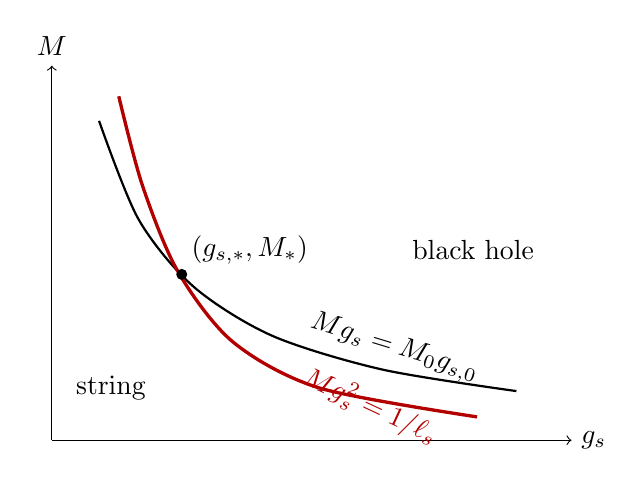
\begin{tikzpicture}[x=1cm,y=0.78cm]
  \draw[->] (0.4,0.4)--(7.0,0.4) node[right] {\(g_s\)};
  \draw[->] (0.4,0.4)--(0.4,6.5) node[above] {\(M\)};
  \draw[thick,black] plot[smooth] coordinates {(1.0,5.6) (1.5,4.0) (2.2,2.9) (3.2,2.1) (4.6,1.55) (6.3,1.2)};
  \draw[very thick,red!70!black] plot[smooth] coordinates {(1.25,6.0) (1.55,4.55) (2.0,3.15) (2.7,2.0) (3.8,1.25) (5.8,0.78)};
  \fill (2.05,3.1) circle (2pt) node[above right] {\((g_{s,*},M_*)\)};
  \node[black,rotate=-17] at (4.75,1.9) {\(Mg_s=M_0g_{s,0}\)};
  \node[red!70!black,rotate=-25] at (4.45,0.95) {\(Mg_s^2=1/\ell_s\)};
  \node at (5.75,3.5) {black hole};
  \node at (1.15,1.25) {string};
\end{tikzpicture}
\caption{El gráfico de la pizarra y su interpretación depurada. La adiabat negra corta la curva de correspondencia roja, más pronunciada, en el punto donde el objeto adquiere carácter de cuerda.}
\lectureframe{00:49:35.000}
\end{figure}

En la intersección \((M_*,g_{s,*})\), las dos ecuaciones son
\begin{align}
M_*g_{s,*} &= M_0g_{s,0}, \\
M_*g_{s,*}^2 &\sim \frac{1}{\ell_s}.
\end{align}
Elevemos al cuadrado la primera ecuación y dividamos por la segunda:
\begin{equation}
M_*
\sim M_0^2g_{s,0}^2\ell_s.
\end{equation}
Al multiplicar por \(\ell_s\),
\begin{equation}
M_*\ell_s
\sim M_0^2g_{s,0}^2\ell_s^2
\sim M_0^2G_{N,0}.
\label{eq:l07-crossover-result}
\end{equation}

\begin{figure}[htbp]
\centering
\includegraphics[width=0.68\textwidth]{lecture_07_figure_08.png}
\caption{El álgebra completa de la transición, incluido \(M_*\ell_s=M_0^2g_{s,0}^2\ell_s^2=M_0^2G_{N,0}\).}
\lectureframe{00:54:40.000}
\end{figure}

\begin{classroomqa}
\audiencequestion{Al dividir las ecuaciones de las dos curvas, ¿\(\ell_s\) queda en el numerador o en el denominador?\lecturetimestamp{00:52:41}}
\lecturerresponse{En el numerador. Dividir por \(1/\ell_s\) equivale a multiplicar por \(\ell_s\), y por eso \(M_*\sim M_0^2g_{s,0}^2\ell_s\).}
\end{classroomqa}

En la transición es válida la fórmula de la cuerda, así que
\begin{equation}
S_*\sim M_*\ell_s.
\end{equation}
La entropía no cambió a lo largo de la trayectoria. Al combinar esta afirmación con la ecuación~\eqref{eq:l07-crossover-result} obtenemos la entropía del agujero negro objetivo original:
\begin{equation}
S_{\mathrm{BH}}(M_0)
\sim M_0^2G_{N,0}
\sim M_0^2\ell_{p,0}^2.
\label{eq:l07-final-correspondence}
\end{equation}
Esta es la dependencia deseada según la ley del área.

\section{Qué demuestra y qué no demuestra la correspondencia}

Esta construcción no afirma que el agujero negro original, con su intensa gravedad, sea una cuerda libre. Lleva el objeto a un régimen donde el recuento de cuerdas es fiable, obtiene allí la entropía y la transporta de vuelta a lo largo de una trayectoria reversible. La transición es un cruce gradual, no una frontera de fase claramente definida, así que esta estimación no permite determinar el coeficiente \(1/4\) de la ecuación~\eqref{eq:l07-bh-exact}.

El mismo razonamiento funciona, no obstante, de forma paramétrica para los agujeros negros cargados, los objetos negros en otras dimensiones y las branas negras extendidas. En ejemplos con más simetría y supersimetría se pueden contar estados protegidos que conservan información exacta al variar el acoplamiento; esos métodos recuperan los coeficientes numéricos, pero requieren herramientas matemáticas que no hacen falta para el argumento conceptual de hoy.

Lo más importante es que el cálculo proporciona una interpretación microscópica. La entropía es una señal de que existe una estructura oculta. La mecánica de fluidos describe densidad, presión y flujo sin mostrar las moléculas; la entropía del fluido revela la existencia de esos grados de libertad microscópicos. De manera similar, la relatividad general describe un horizonte sin mostrar sus microestados. El recuento de cuerdas muestra que una teoría cuántica coherente de la gravedad puede contener suficientes estados para dar cuenta de la entropía de los agujeros negros.

\begin{classroomqa}
\audiencequestion{¿Qué habría significado \(S\sim M^3\ell_p^3\), en lugar del resultado cuadrático?\lecturetimestamp{00:59:41}}
\lecturerresponse{Habría tenido la forma de una ley de volumen. La entropía de la materia ordinaria en una habitación o en una taza de café es proporcional al volumen; la respuesta cuadrática es especial porque, mediante \(R_s\sim M\ell_p^2\), es proporcional al área del horizonte.}
\end{classroomqa}

El resultado indica que la entropía de Bekenstein--Hawking no es una mera analogía termodinámica formal. Apunta a grados de libertad gravitatorios microscópicos, aunque la derivación elemental no los haga visibles uno por uno.

\section{De la entropía máxima a la holografía}

Ahora cambiamos de pregunta. En vez de preguntar por la entropía de un estado dado, preguntamos cuál es la entropía máxima compatible con una región.

Empecemos con un modelo reticular corriente de una habitación. Dividamos el volumen en celdas de tamaño \(V_{\mathrm{cell}}\) y asignemos a cada celda una pregunta de sí o no: ¿está ocupada o vacía? Susskind da al átomo imaginario el nombre deliberadamente absurdo de ``meatonium'', para que ningún detalle atómico realista distraiga del recuento. Si
\begin{equation}
N=\frac{V}{V_{\mathrm{cell}}},
\end{equation}
entonces el número de configuraciones y la entropía máxima son
\begin{equation}
\Omega=2^N,
\qquad
S_{\max}=\log\Omega=N\log2
\sim\frac{V}{V_{\mathrm{cell}}}.
\label{eq:l07-volume-count}
\end{equation}

\begin{figure}[htbp]
\centering
\includegraphics[width=0.68\textwidth]{lecture_07_figure_09.png}
\caption{La habitación, dividida en celdas, con dos estados por celda. Esto cuenta la entropía máxima, no la entropía de la habitación ordenada que ocupa la clase.}
\lectureframe{01:05:20.000}
\end{figure}

La habitación real está muy por debajo de este máximo. Un estado que recorriera caóticamente todas esas opciones de las celdas estaría extremadamente caliente. Lo que se conserva del modelo simplificado es la expectativa habitual de que el número de grados de libertad independientes y, por tanto, la entropía máxima escalan con el volumen.

La gravedad trastoca esa expectativa. Consideremos una región esférica de área de frontera \(A\), entropía inicial \(S_{\mathrm{i}}\) y masa \(M\), menor que la masa \(M_{\mathrm{BH}}\) de un agujero negro que llenaría justo la esfera. Si \(M\) fuera mayor, su horizonte ya se extendería más allá de la frontera elegida.

Enviemos ahora una capa esférica de masa \(M_{\mathrm{BH}}-M\). Su composición es irrelevante: la clase contempla que sea de luz, de materia ordinaria o incluso de queso suizo. Dispongamos que colapse. El estado final es un agujero negro cuyo horizonte llena justo la región y cuya entropía es
\begin{equation}
S_{\mathrm{f}}=\frac{A}{4G_N}.
\end{equation}
La segunda ley exige que
\begin{equation}
S_{\mathrm{i}}\le S_{\mathrm{f}}
=\frac{A}{4G_N}.
\label{eq:l07-holographic-bound}
\end{equation}

\begin{figure}[htbp]
\centering
\includegraphics[width=0.70\textwidth]{lecture_07_figure_10.png}

\vspace{0.5em}
\begin{tikzpicture}[scale=0.88]
  \draw[thick] (0,0) circle (1.35);
  \draw[very thick,red!70!black] (0,0) circle (2.05);
  \fill[gray!25] (0,0) circle (1.32);
  \node at (0,0) {\(M,S_{\mathrm{i}}\)};
  \draw[-{Latex[length=3mm]},thick,red!70!black] (3.5,0)--(2.15,0);
  \node[align=center,right] at (3.5,0) {incoming shell\\\(M_{\mathrm{BH}}-M\)};
  \node[below] at (0,-2.2) {final horizon area \(A\)};
\end{tikzpicture}
\caption{La construcción con la capa esférica. Se envía hacia dentro masa adicional suficiente para formar un agujero negro cuyo horizonte llena justo la región seleccionada.}
\lectureframe{01:13:30.000}
\end{figure}

Como un agujero negro de ese tamaño es un estado permitido y satura la desigualdad, la entropía máxima es
\begin{equation}
S_{\max}=\frac{A}{4G_N}.
\label{eq:l07-holographic-maximum}
\end{equation}
Esta es la formulación en términos de recuento del principio holográfico: el número máximo de grados de libertad independientes en una región gravitatoria escala con el área de su frontera; en orden de magnitud, corresponde a un grado de libertad por área de Planck, y no al número de volúmenes de Planck interiores.\editorialnote{El argumento de la capa esférica supone que la región puede encerrarse y colapsar de la manera indicada. Los espaciotiempos más generales requieren cotas covariantes de entropía, pero el argumento esférico recoge el principio empleado en la clase.}

La diferencia es enorme. La intuición de la teoría de campos local sugiere que las elecciones hechas en distintos puntos interiores deberían combinarse de forma independiente y producir una ley de volumen. La gravedad dice que un número suficiente de esas elecciones se colapsaría por sí solo, y el agujero negro ofrece la entropía admisible máxima. Por tanto, el recuento de frontera no es una pequeña corrección al recuento de volumen: supone una organización distinta del espacio de Hilbert.

\begin{classroomqa}
\audiencequestion{¿Qué ocurre en un universo muy grande con una densidad aproximadamente uniforme?\lecturetimestamp{01:15:48}}
\lecturerresponse{Esa pregunta requiere cosmología, no la construcción esférica estática. Motiva el paso inmediato a las soluciones en expansión de las ecuaciones de Einstein.}
\end{classroomqa}

\begin{classroomqa}
\audiencequestion{¿Está relacionada la cota del área con el principio de incertidumbre?\lecturetimestamp{01:16:03}}
\lecturerresponse{La clase deja esta pregunta abierta y pasa a la cosmología.}
\end{classroomqa}

\section{El espacio en expansión}

Aquí no deduciremos las soluciones cosmológicas a partir de las ecuaciones de Einstein; las escribiremos y aprenderemos a interpretarlas. Las secciones espaciales pueden tener curvatura positiva y ser cerradas, curvatura negativa y ser hiperbólicas, o ser planas. Para esta explicación consideremos secciones espaciales euclidianas planas en un espaciotiempo dependiente del tiempo.

\begin{classroomqa}
\audiencequestion{¿Cuál es el análogo espaciotemporal del espacio euclidiano ordinario?\lecturetimestamp{01:19:37}}
\lecturerresponse{El espacio de Minkowski. La cosmología que consideramos aquí tiene secciones espaciales planas, pero no es un espaciotiempo de Minkowski, porque su métrica espacial cambia con el tiempo.}
\end{classroomqa}

La conocida imagen del globo describe una superficie cerrada en expansión y de una dimensión menos. Susskind recuerda que intentó hacer la demostración con un globo grande marcado; el rotulador debilitó la goma y provocó un estallido literal. El percance también pone al descubierto un defecto conceptual de la analogía. Cuando un globo ordinario se expande, sus moléculas de goma se separan y el material se adelgaza hasta romperse. En el espacio cosmológico, las leyes locales no se diluyen. Para que la analogía funcione, hay que imaginar que se insertan continuamente moléculas de goma nuevas, de modo que cada pequeña zona conserve las mismas propiedades locales. En un modelo plano, sustituyamos el globo por una gran lámina que se estira uniformemente y se repone de manera análoga.

Matemáticamente, la expansión se incorpora a la métrica:
\begin{equation}
\begin{aligned}
ds^2&=-dt^2+a(t)^2d\mathbf{x}^2,\\
d\mathbf{x}^2&=\delta_{ij}\,dx^i dx^j
=dx^2+dy^2+dz^2.
\end{aligned}
\label{eq:l07-frw-metric}
\end{equation}

\begin{figure}[htbp]
\centering
\includegraphics[width=0.72\textwidth]{lecture_07_figure_11.png}
\caption{La métrica de expansión espacial plana tal como está escrita en la pizarra.}
\lectureframe{01:25:10.000}
\end{figure}

Los puntos cuyas coordenadas espaciales permanecen fijas se llaman comóviles. Si dos puntos comóviles tienen una separación coordenada \(\Delta x\), su distancia propia en el instante \(t\) es
\begin{equation}
D(t)=a(t)\Delta x.
\label{eq:l07-proper-distance}
\end{equation}
Sus coordenadas no cambian, pero sí cambia la distancia métrica entre ellos. Al derivar manteniendo fijo \(\Delta x\),
\begin{equation}
V=\dot D=\dot a\,\Delta x
=\frac{\dot a}{a}D.
\end{equation}
Definamos el parámetro de Hubble
\begin{equation}
H(t)=\frac{\dot a(t)}{a(t)}.
\label{eq:l07-hubble-parameter}
\end{equation}
Entonces,
\begin{equation}
V=H(t)D,
\label{eq:l07-hubble-law}
\end{equation}
que es la ley de Hubble en un instante cósmico fijo.

\begin{figure}[htbp]
\centering
\includegraphics[width=0.68\textwidth]{lecture_07_figure_12.png}
\caption{La ley de recesión a tiempo igual escrita en la pizarra: \(V=D\,\dot a/a\).}
\lectureframe{01:29:10.000}
\end{figure}

La expresión ``constante de Hubble'' puede llevar a confusión. En general, \(H(t)\) cambia con el tiempo. Lo que es constante espacialmente es la razón \(V/D\) para cada par de puntos comóviles en una misma sección temporal.

\begin{classroomqa}
\audiencequestion{En el caso de las galaxias lejanas, ¿a qué instante corresponde el tiempo de esta relación? Las observamos en una época anterior.\lecturetimestamp{01:31:10}}
\lecturerresponse{La ecuación~\eqref{eq:l07-hubble-law} es una afirmación válida a tiempo igual. Una observación sigue un rayo de luz dirigido hacia el pasado y, por ello, detecta la galaxia lejana en un instante anterior. Así que la relación entre el corrimiento al rojo medido y la distancia requiere conocer toda la historia del cono de luz, no un único valor instantáneo de \(H\).}
\end{classroomqa}

\begin{figure}[htbp]
\centering
\includegraphics[width=0.66\textwidth]{lecture_07_figure_13.png}
\caption{El esquema espaciotemporal empleado para distinguir una separación a tiempo igual de lo que observa alguien a lo largo de un rayo de luz dirigido hacia el pasado.}
\lectureframe{01:33:20.000}
\end{figure}

\section{La escala de Hubble y la expansión de de Sitter}

En unidades \(c=1\), la ecuación~\eqref{eq:l07-hubble-law} asigna una velocidad de recesión igual a la velocidad de la luz a la distancia
\begin{equation}
D_H=\frac{1}{H}.
\label{eq:l07-hubble-radius}
\end{equation}
Puntos comóviles más lejanos pueden tener \(V>1\), e incluso \(V\gg1\), sin violar la relatividad especial. No pasan junto a un observador local a una velocidad mayor que la de la luz: su separación propia aumenta porque se expande la geometría intermedia.\editorialnote{En una cosmología general dependiente del tiempo, \(1/H\) es el radio de Hubble, pero no es automáticamente un horizonte de sucesos. En el caso de de Sitter que veremos a continuación, sí es la escala constante del horizonte.}

En muchos modelos cosmológicos antiguos con expansión desacelerada, \(H(t)\) disminuye y \(1/H(t)\) aumenta, de modo que regiones que antes se alejaban a velocidad superlumínica pueden entrar más tarde en contacto causal. En cambio, la imagen de tiempos tardíos que se analiza en la clase se aproxima a un valor positivo constante \(H\). Entonces \(1/H\) permanece fijo y la ecuación de expansión pasa a ser
\begin{equation}
\frac{\dot a}{a}=H,
\qquad
\dot a=Ha.
\label{eq:l07-constant-h}
\end{equation}

\begin{classroomqa}
\audiencequestion{¿Qué unidades tiene un parámetro de Hubble constante?\lecturetimestamp{01:38:24}}
\lecturerresponse{El inverso del tiempo. De manera equivalente, cuando \(c=1\), es el inverso de una longitud. La magnitud \(H^{-1}\) proporciona tanto una escala temporal de expansión como una escala de distancia; la clase usa como ejemplo un valor aproximado de quince mil millones de años.}
\end{classroomqa}

La solución de la ecuación~\eqref{eq:l07-constant-h} es
\begin{equation}
a(t)=a_0e^{Ht}.
\label{eq:l07-desitter-scale-factor}
\end{equation}

\begin{classroomqa}
\audiencequestion{¿Qué función tiene una tasa de variación proporcional a sí misma?\lecturetimestamp{01:39:04}}
\lecturerresponse{Una exponencial. Por tanto, el factor de escala es \(a_0e^{Ht}\), mientras que el coeficiente espacial \(a(t)^2\) de la métrica crece como \(e^{2Ht}\).}
\end{classroomqa}

\begin{figure}[htbp]
\centering
\includegraphics[width=0.70\textwidth]{lecture_07_figure_14.png}
\caption{Las ecuaciones con \(H\) constante y su solución exponencial, escritas en la pizarra.}
\lectureframe{01:39:30.000}
\end{figure}

Un espaciotiempo con esta expansión exponencial es el espacio de de Sitter. Su escala de Hubble constante produce un horizonte de sucesos a una distancia propia finita. En cierto sentido, esta geometría complementa la imagen del agujero negro: un observador permanece dentro de un horizonte cosmológico, mientras los objetos suficientemente lejanos se alejan y nunca pueden enviar señales que alcancen al observador. El horizonte de un agujero negro oculta el interior a un observador exterior; el horizonte de de Sitter oculta el exterior de la región accesible al observador. A diferencia de un agujero negro ordinario que se evapora, aquí se considera que la geometría ideal de de Sitter persiste. Aquí apenas comienza la comparación. La siguiente clase desarrolla el horizonte, su termodinámica y los enigmas que plantea para la cosmología.
